% !TEX TS-program = pdflatexmk

\documentclass[14pt]{beamer}
\usepackage{newtxtext,newtxmath}
\usepackage{microtype}
\usepackage[english]{babel}
\usepackage{hyperref}
\usepackage{graphicx}
\usepackage{listings}
\lstloadlanguages{Python}
\lstset{language=Python}
\lstset{%
basicstyle=\ttfamily\bfseries,
keywordstyle=\color{blue}, emph={self}, emphstyle={\color{blue}},
identifierstyle=,
commentstyle=\color{brown},
stringstyle=\color{green!50!black},
showstringspaces=false,
emphstyle={[2]\color{purple}},
}
\usepackage{tikz}
\usepackage{forest}
\usetikzlibrary{positioning}
\usepackage{array}
\newcolumntype{L}[1]{>{\raggedright\let\newline\\\arraybackslash\hspace{0pt}}m{#1}}

\mode<presentation>{
\usetheme{Madrid}
\definecolor{uabgreen}{cmyk}{.89,.31,.78,.17}
\usecolortheme[named=uabgreen]{structure}
\setbeamertemplate{navigation symbols}{}
\setbeamertemplate{footline}[frame number]
\setbeamertemplate{section in toc}[square]
\setbeamertemplate{subsection in toc}[square]
\setbeamertemplate{items}[square]
\setbeamercovered{transparent=5}
}

\newcommand{\keyword}[1]{{\color{blue}#1}}
\newcommand{\cmnt}[1]{{\color{gray}#1}}
\newcommand{\str}[1]{{\color{green!50!black}#1}}
\newcommand{\defn}[1]{{\color{purple}#1}}

\author[Dr. Bethard]{Dr. Steven Bethard}
\institute[UAB CIS]{%
Computer and Information Sciences\\
University of Alabama at Birmingham}

\AtBeginSection[]
{
  \begin{frame}<beamer>{Outline}
    \tableofcontents[currentsection]
  \end{frame}
}

\tikzset{
  invisible/.style={opacity=0,text opacity=0},
  visible on/.code={%
    \alt<#1>{}{\pgfkeysalso{invisible}}
  },
  filled on/.code={%
    \alt<#1>{\pgfkeysalso{fill=gray}}{}
  },
}
\forestset{
  edge weight/.style={
    edge label={node[midway,above,sloped]{#1}}},
  invisible/.style={
    /tikz/invisible,
    edge={/tikz/invisible}},
  visible on filled on/.code n args={2}{%
    \alt<#1>{\alt<#2>{\pgfkeysalso{fill=gray}}{}}{\pgfkeysalso{invisible}}
  },
  visible on/.code={%
    \alt<#1>{}{\pgfkeysalso{invisible}}
  },
}

\lstset{emph={[2]__init__,__str__,take_action,ProblemSolvingAgent,tree_search,graph_search}}
\newcommand{\key}[1]{\mbox{\texttt{\bfseries\color{red}#1}}}

\title{Solving Problems by Searching}
\date[]{9 Jan 2014}

\begin{document}

\begin{frame}
  \titlepage
\end{frame}

\part{Solving Problems by Searching}

\begin{frame}{Outline}
\tableofcontents
\end{frame}

\section{Search Problems}

\subsection{Properties of Search Problems}
\begin{frame}[plain]
	\begin{center}
		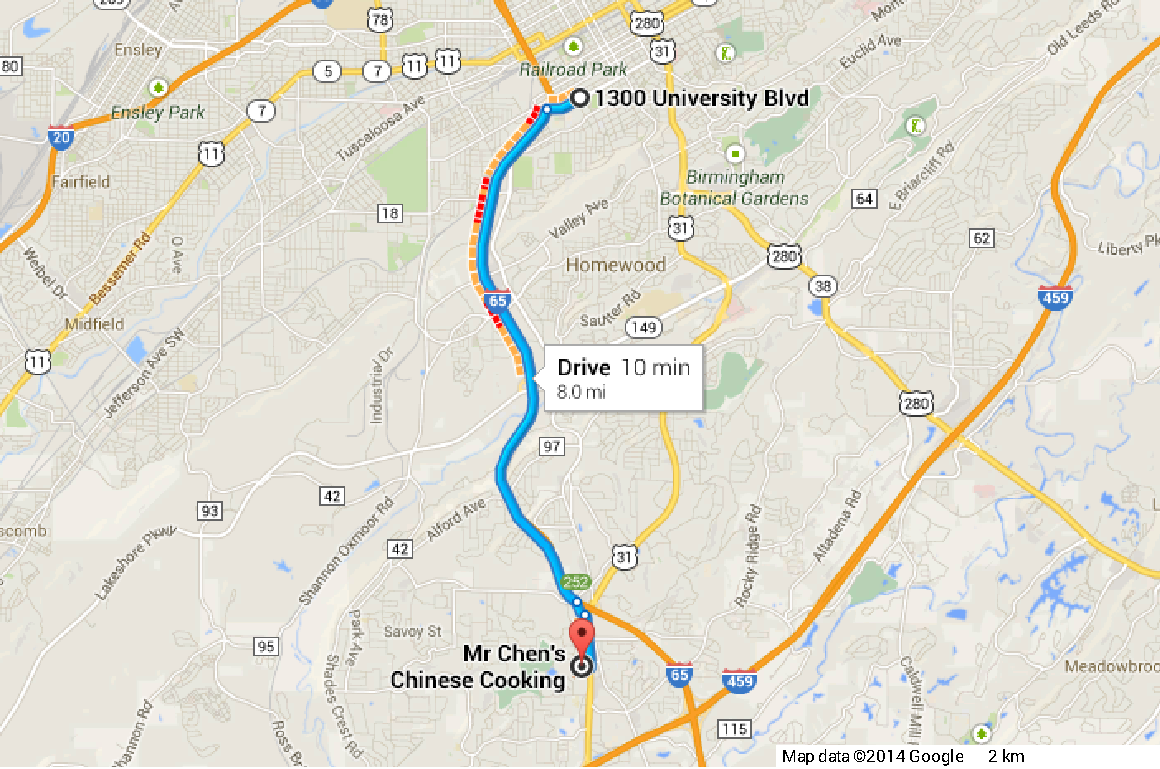
\includegraphics[width=\textwidth]{uab-to-mr-chens.pdf}
	\end{center}
\end{frame}

\begin{frame}{Properties of Search Problems}
	\begin{itemize}
		\item \alert<2->{Fully} or Partially Observable?
		\item \alert<2->{Deterministic} or Stochastic?
		\item Episodic or \alert<2->{Sequential}?
		\item \alert<2->{Static} or Dynamic?
		\item \alert<2->{Discrete} or Continuous?
		\item \alert<2->{Single} or Multi-Agent?
	\end{itemize}
\end{frame}

\begin{frame}{Example: Vacuum Problem}
	\begin{columns}
		\column{.50\textwidth}
			\begin{block}{Problem}
				\begin{itemize}
					\item Start in \key{1}
					\item Left square actions:\\
					      \key{Suck} or \key{Right}
					\item Right square actions:\\
					      \key{Suck} or \key{Left}
					\item Success: \key{7} or \key{8}
					\item Optimal: fewest actions
				\end{itemize}
			\end{block}
			\begin{block}{Solution}<2->
				\uncover<3->{[\key{Suck}, \key{Right}, \key{Suck}]} \\
				\uncover<4->{i.e., [\key{1}, \key{5}, \key{6}, \key{8}]}
			\end{block}
		\column{.50\textwidth}
			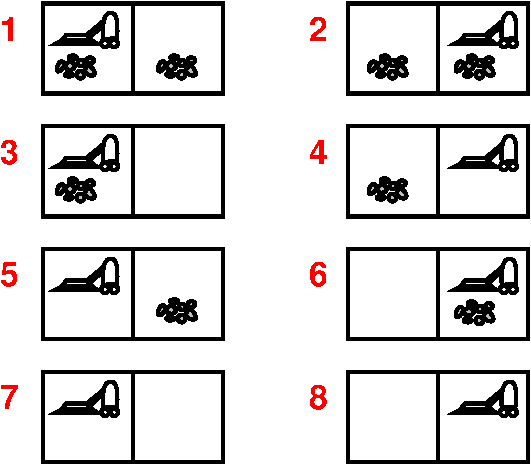
\includegraphics[width=2.1in]{vacuum-space.pdf}
	\end{columns}
\end{frame}

\begin{frame}{Defining a Search Problem}
	\begin{block}{Components}
		\begin{itemize}
			\item Initial state
			\item Actions
			\item Goal test
			\item Path cost
		\end{itemize}
	\end{block}
	\begin{block}{Solution}
		Path from initial state to goal state
	\end{block}
	\begin{block}{Optimal solution}
		Path with lowest cost
	\end{block}
\end{frame}

\begin{frame}{Defining the Vacuum Problem}
	\begin{columns}
		\column{.45\textwidth}
			\begin{block}{Initial State}
				\key{1}
			\end{block}
			\begin{block}{Actions}
				\small
	      $S(\key{1}) = \{(\key{Right}, \key{2}), (\key{Suck}, \key{5})\}$ \\
	      $S(\key{2}) = \{(\key{Left}, \key{1}), (\key{Suck}, \key{4})\}$ \\
	      \ldots
			\end{block}
			\begin{block}{Goal Test}
				$G(s) = s \in \{\key{7}, \key{8}\}$
			\end{block}
			\begin{block}{Path Cost}
				1 per state
			\end{block}
		\column{.50\textwidth}
			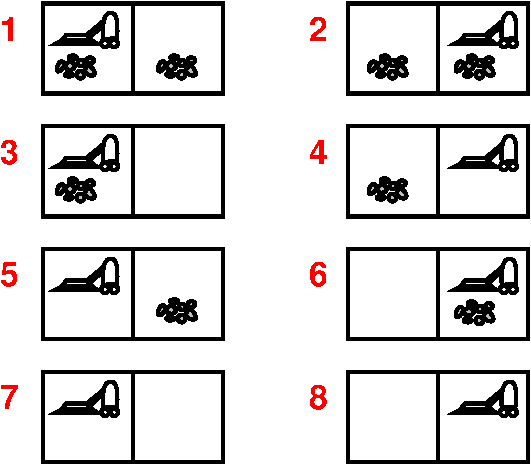
\includegraphics[width=2.1in]{vacuum-space.pdf}
	\end{columns}
\end{frame}

\subsection{Search Problem Examples}
\begin{frame}{Defining the 8-Puzzle Problem}
	\begin{center}
		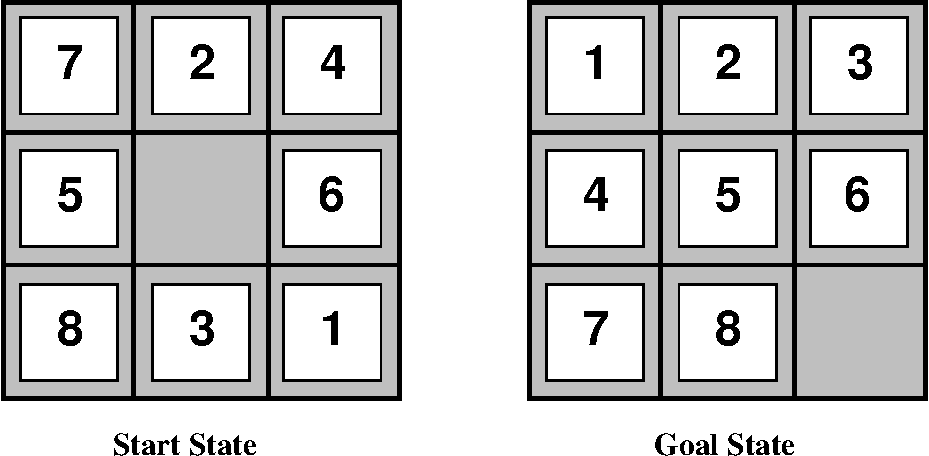
\includegraphics[height=1.5in]{8puzzle.pdf}
	\end{center}
	\begin{description}
		\item[States] \uncover<2->{Mappings of tile numbers to tile locations }
		\item[Initial] \uncover<3->{$\{
			1\!\!:\!\!9,
			2\!\!:\!\!2,
			3\!\!:\!\!8,
			4\!\!:\!\!3,
			5\!\!:\!\!4,
			6\!\!:\!\!6,
			7\!\!:\!\!1,
			8\!\!:\!\!9\}$}
		\item[Actions] \uncover<4->{Move blank left, right, up, down}
		\item[Goal] \uncover<5->{$\{
			1\!\!:\!\!1,
			2\!\!:\!\!2,
			3\!\!:\!\!3,
			4\!\!:\!\!4,
			5\!\!:\!\!5,
			6\!\!:\!\!6,
			7\!\!:\!\!7,
			8\!\!:\!\!8\}$}
		\item[Cost] \uncover<6->{1 per move}
	\end{description}
\end{frame}

\begin{frame}{Defining the Robotic Assembly Problem}
	\begin{center}
		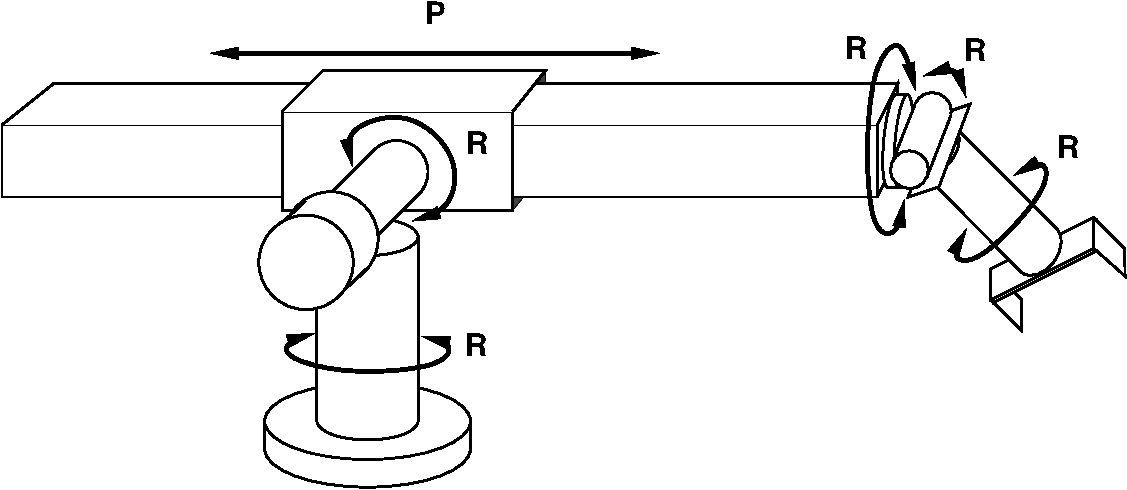
\includegraphics[height=1.5in]{stanford-arm.pdf}
	\end{center}
	\begin{description}
		\item[States] \uncover<2->{real-valued joint angles, parts to assemble}
		\item[Initial] \uncover<3->{many possible}
		\item[Actions] \uncover<4->{real-valued adjustments to joint angles}
		\item[Goal] \uncover<5->{fully assembled part}
		\item[Cost] \uncover<6->{total duration of all movements}
	\end{description}
\end{frame}

\begin{frame}{Defining the Machine Translation Problem}
	\begin{description}
		\item[Input] Com\'i la manzana roja porque ten\'ia hambre.
		\item[Output] I ate the red apple because I was hungry.
		\bigskip\bigskip
		\item[States]
		\item[Initial]
		\item[Actions]
		\item[Goal]
		\item[Cost]
	\end{description}
\end{frame}

\section{Search Algorithms}

\subsection{Search Trees}

\begin{frame}[fragile]{Tree Search}
	\footnotesize
	\begin{lstlisting}
		def tree_search(problem, strategy):

		    strategy.add(...problem.initial_state...)

		    for node in strategy:

		        if problem.is_goal(node.state):
		            return node.get_actions()

		        items = problem.get_successors(node.state)
		        for state, action, ... in items:
		            strategy.add(...state...action...)

		    return None
	\end{lstlisting}
\end{frame}

\begin{frame}{Search Tree Example}
\begin{center}
\small
\pgfkeys{/pgf/inner sep=0.25em}
\begin{forest}
for tree={grow'=east,l sep=4em}
[Birmingham
  [Atlanta,visible on={2-}
    [Birmingham,visible on={3-}]
    [Chattanooga,visible on={3-}]
    [Augusta,visible on={3-}]
    [\ldots,visible on={3-}]
  ]
  [Montgomery,visible on={2-}
    [Birmingham,visible on={4-}]
    [Atlanta,visible on={4-}]
    [Mobile,visible on={4-}]
    [\ldots,visible on={4-}]
  ]
  [Tuscaloosa,visible on={2-}
    [Birmingham,visible on={5-}]
    [Meridian,visible on={5-}]
    [Starkville,visible on={5-}]
    [\ldots,visible on={5-}]
  ]
]
\end{forest}
\end{center}
\end{frame}

\subsection{Search Nodes}

\begin{frame}{The Node Data Structure}
	\begin{center}
		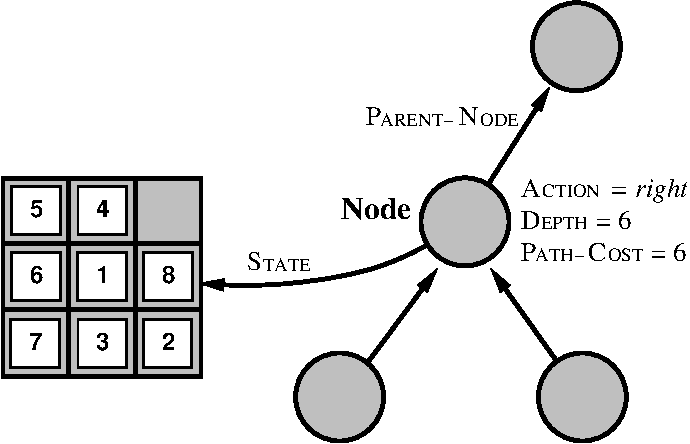
\includegraphics[width=4in]{state-vs-node.pdf}
	\end{center}
\end{frame}

\begin{frame}[fragile]{Tree Search Revisited}
	\footnotesize
	\begin{lstlisting}
		def tree_search(problem, strategy):
		    strategy.add(Node(problem.initial_state))
		    for node in strategy:
		        if problem.is_goal(node.state):
		            return node.get_actions()
		        succs = problem.get_successors(node.state)
		        for state, action, cost in succs:
		            strategy.add(Node(
		                state=state,
		                action=action,
		                parent=node,
		                cost=node.cost + cost,
		                depth=node.depth + 1))
		    return None
	\end{lstlisting}
\end{frame}

\section{Search Strategies}
\begin{frame}[<+->]{Search Strategy Properties}
	\begin{block}{Completeness}
		If a solution exists, is it always found?
	\end{block}
	\begin{block}{Optimality}
		Is the solution found always the lowest cost?
	\end{block}
	\begin{block}{Time Complexity}
		How many search nodes will be generated?
	\end{block}
	\begin{block}{Space Complexity}
		How many search nodes must stay in main memory?
	\end{block}
\end{frame}

\subsection{Breadth-first Search}
\begin{frame}[label=breadth-first-example]{Breadth-first Search}
\begin{center}
\begin{forest}
for tree={circle,draw}
[A,visible on filled on={1-}{2-}
  [B,visible on filled on={2-}{3-}
    [D,visible on filled on={3-}{5-}
      [H,visible on={5-}]
      [I,visible on={5-}]
    ]
    [E,visible on filled on={3-}{6-}
      [J,visible on={6-}]
      [K,visible on={6-}]
    ]
  ]
  [C,visible on filled on={2-}{4-}
    [F,visible on filled on={4-}{7-}
      [L,visible on={7-}]
      [M,visible on={7-}]
    ]
    [G,visible on={4-}
      [N,invisible]
      [O,invisible]
    ]
  ]
]
\end{forest}
\end{center}
\end{frame}
\begin{frame}{Breadth-first Properties}
	\footnotesize
	\begin{block}{Strategy? \hyperlink{breadth-first-example}{\beamergotobutton{Example}}}
		 \uncover<2->{First-in First-Out Queue}
	\end{block}
	\begin{block}{Complete?}
		\uncover<3->{Yes, if number of branches is finite}
	\end{block}
	\begin{block}{Optimal?}
		\uncover<4->{Yes, if step costs are all identical}
	\end{block}
	\begin{block}{Worst Case Time Complexity?}
		\uncover<5->{$O(b^{d+1})$, branching factor $b$, depth of goal state $d$}
	\end{block}
	\begin{block}{Worst Case Space Complexity?}
		\uncover<6->{$O(b^{d+1})$, branching factor $b$, depth of goal state $d$}
	\end{block}
\end{frame}

\subsection{Uniform-cost Search}
\begin{frame}[label=uniform-cost-example]{Uniform-cost Search}
\begin{center}
\begin{forest}
for tree={circle,draw},
[A,visible on filled on={1-}{2-}
  [B,edge weight={2},visible on filled on={2-}{4-}
    [D,edge weight={1},visible on filled on={4-}{6-}
      [H,edge weight={2},visible on={6-}]
      [I,edge weight={3},visible on={6-}]
    ]
    [E,edge weight={1},visible on={4-}
      [J,edge weight={3},invisible]
      [K,edge weight={2},invisible]
    ]
  ]
  [C,edge weight={1},visible on filled on={2-}{3-}
    [F,edge weight={3},visible on={3-}
      [L,edge weight={1},invisible]
      [M,edge weight={1},invisible]
    ]
    [G,edge weight={2},visible on filled on={3-}{5-}
      [N,edge weight={1},visible on={5-}]
      [O,edge weight={3},visible on={5-}]
    ]
  ]
]
\end{forest}
\end{center}
\end{frame}
\begin{frame}{Uniform-cost Search}
	\footnotesize
	\begin{block}{Strategy? \hyperlink{uniform-cost-example}{\beamergotobutton{Example}}}
		\uncover<2->{Lowest Cost First Priority Queue}
	\end{block}
	\begin{block}{Complete?}
		\uncover<3->{Yes, if number of branches is finite and steps are all positive}
	\end{block}
	\begin{block}{Optimal?}
		\uncover<4->{Yes}
	\end{block}
	\begin{block}{Worst Case Time Complexity?}
		\uncover<5->{$O(b^{\left\lfloor C^{*}/\epsilon \right\rfloor +1})$, optimal cost $C^{*}$, minimum step cost $\epsilon$}
	\end{block}
	\begin{block}{Worst Case Space Complexity?}
		\uncover<6->{$O(b^{\left\lfloor C^{*}/\epsilon \right\rfloor +1})$, optimal cost $C^{*}$, minimum step cost $\epsilon$}
	\end{block}
\end{frame}

\subsection{Depth-first Search}
\begin{frame}[label=depth-first-example]{Depth-first Search}
\begin{center}
\begin{forest}
for tree={circle,draw}
[A,visible on filled on={1-}{2-}
  [B,visible on filled on={2-9}{3-}
    [D,visible on filled on={3-6}{4-}
      [H,visible on filled on={4-5}{5-}]
      [I,visible on filled on={4-6}{6-}]
    ]
    [E,visible on filled on={3-9}{7-}
      [J,visible on filled on={7-8}{8-}]
      [K,visible on filled on={7-9}{9-}]
    ]
  ]
  [C,visible on={2-10}
    [F,invisible
      [L,invisible]
      [M,invisible]
    ]
    [G,invisible
      [N,invisible]
      [O,invisible]
    ]
  ]
]
\end{forest}
\end{center}
\end{frame}
\begin{frame}{Depth-first Properties}
	\footnotesize
	\begin{block}{Strategy? \hyperlink{depth-first-example}{\beamergotobutton{Example}}}
		\uncover<2->{First-in Last-Out Stack}
	\end{block}
	\begin{block}{Complete?}
		\uncover<3->{Yes, if finite number of states and no cyclic paths}
	\end{block}
	\begin{block}{Optimal?}
		\uncover<4->{No, lower goal states may be found first}
	\end{block}
	\begin{block}{Worst Case Time Complexity?}
		\uncover<5->{$O(b^{m})$, branching factor $b$, maximum depth $m$}
	\end{block}
	\begin{block}{Worst Case Space Complexity?}
		\uncover<6->{$O(bm)$, branching factor $b$, maximum depth $m$}
	\end{block}
\end{frame}

\subsection{Iterative Deepening Search}
\begin{frame}[label=iterative-deepening-example]{Iterative Deepening Search}
\begin{center}
\begin{forest}
for tree={circle,draw}
[A,visible on filled on={1-2,4-7,9-16,18}{2,5-7,10-16}
  [B,visible on filled on={5-6,10-13}{6,11-13}
    [D,visible on filled on={11-12}{12}
      [H,invisible]
      [I,invisible]
    ]
    [E,visible on filled on={11-13}{13}
      [J,invisible]
      [K,invisible]
    ]
  ]
  [C,visible on filled on={5-7,10-16}{7,14-16}
    [F,visible on filled on={14-15}{15}
      [L,invisible]
      [M,invisible]
    ]
    [G,visible on filled on={14-16}{16}
      [N,invisible]
      [O,invisible]
    ]
  ]
]
\end{forest}
\end{center}
\end{frame}
\begin{frame}{Iterative Deepening Properties}
	\footnotesize
	\begin{block}{Strategy? \hyperlink{iterative-deepening-example}{\beamergotobutton{Example}}}
		\uncover<2->{First-in Last-Out Stack with depth limit}
	\end{block}
	\begin{block}{Complete?}
		\uncover<3->{Yes, if number of branches is finite}
	\end{block}
	\begin{block}{Optimal?}
		\uncover<4->{Yes, if step costs are all identical}
	\end{block}
	\begin{block}{Worst Case Time Complexity?}
		\uncover<5->{$O(b^{d})$, branching factor $b$, depth of goal state $d$}
	\end{block}
	\begin{block}{Worst Case Space Complexity?}
		\uncover<6->{$O(bd)$, branching factor $b$, depth of goal state $d$}
	\end{block}
\end{frame}

\section{Advanced Search}

\subsection{Repeated States}
\begin{frame}{Exponential Costs of Repeated States}
	\begin{center}
		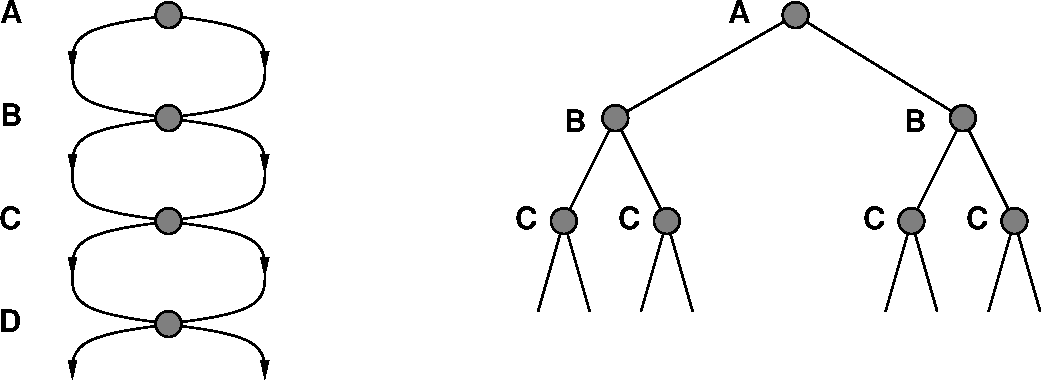
\includegraphics[width=4in]{ribbon-space.pdf}
	\end{center}
\end{frame}
\begin{frame}[fragile]{Graph Search}
	\scriptsize
	\begin{lstlisting}
		def graph_search(problem, strategy):
		    seen = set()
		    strategy.add(Node(problem.initial_state))
		    for node in strategy:
		        if problem.is_goal(node.state):
		            return node.get_actions()
		        if node not in seen:
		            seen.add(node)
		            succs = problem.get_successors(node.state)
		            for state, action, cost in succs:
		                strategy.add(Node(
		                    state=state,
		                    action=action,
		                    parent=node,
		                    cost=node.cost + cost,
		                    depth=node.depth + 1))
	\end{lstlisting}
\end{frame}

\subsection{Partial Information}
\begin{frame}{Searching with Partial Information}
	\begin{columns}
		\column{.50\textwidth}
			\begin{block}{Problem}
				Start in \alert{any state}
			\end{block}
			\begin{block}{Solution?}
				\footnotesize
				\begin{tabular}{ll}
					\uncover<2->{Initial}     & \uncover<2->{$\{\key{1}, \key{2}, \key{3}, \key{4}, \key{5}, \key{6}, \key{7}, \key{8}\}$} \\
					\uncover<3->{\key{Right}} & \uncover<4->{$\{\key{2}, \key{4}, \key{6}, \key{8}\}$} \\
					\uncover<5->{\key{Suck}}  & \uncover<6->{$\{\key{4}, \key{8}\}$} \\
					\uncover<7->{\key{Left}}  & \uncover<8->{$\{\key{3}, \key{7}\}$} \\
					\uncover<9->{\key{Suck}}  & \uncover<10->{$\{\key{7}\}$} \\
				\end{tabular}
			\end{block}
		\column{.50\textwidth}
			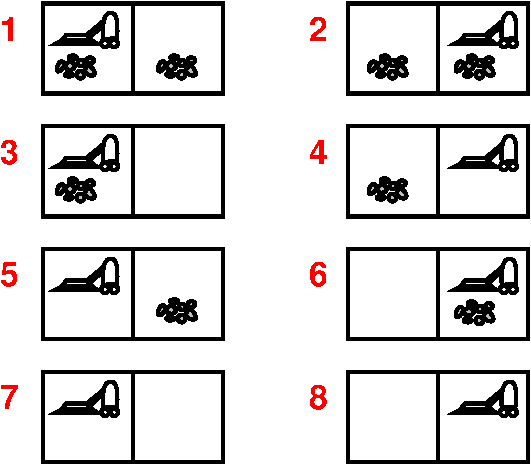
\includegraphics[width=2.1in]{vacuum-space.pdf}
	\end{columns}
\end{frame}

\part{Key Points}
\begin{frame}{Key Points}
	\begin{block}{Search Problems}
		\begin{itemize}
			\item Initial State
			\item Actions
			\item Goal Test
			\item Path Cost
		\end{itemize}
	\end{block}
	\begin{block}{Search Strategies}
		\begin{itemize}
			\item Breadth-first
			\item Uniform-cost
			\item Depth-first
			\item \alert<2->{Iterative Deepening}
		\end{itemize}
	\end{block}
\end{frame}


\end{document}


